\subsection{Overview}

% First use of an acronym: \ac{} prints "Imperial College London (ICL)".
% Later uses: \acs{} prints just "ICL".
Research at \ac{ICL} on \ac{CFD} has a long history \cite{knuthArtComputerProgramming1997,lambPlaceholderJournalArticle2020}. \lipsum[4]

\lipsum[5]

\subsection{Literature Review}

\ac{FEM} approaches \cite{zienkiewiczFiniteElementMethod2013} and finite-volume \acs{CFD} solvers \cite{doeConferencePaperExample2021} are compared in Figure~\ref{fig:sample-cat}. \lipsum[6]

\begin{figure}[ht!]
    \centering
    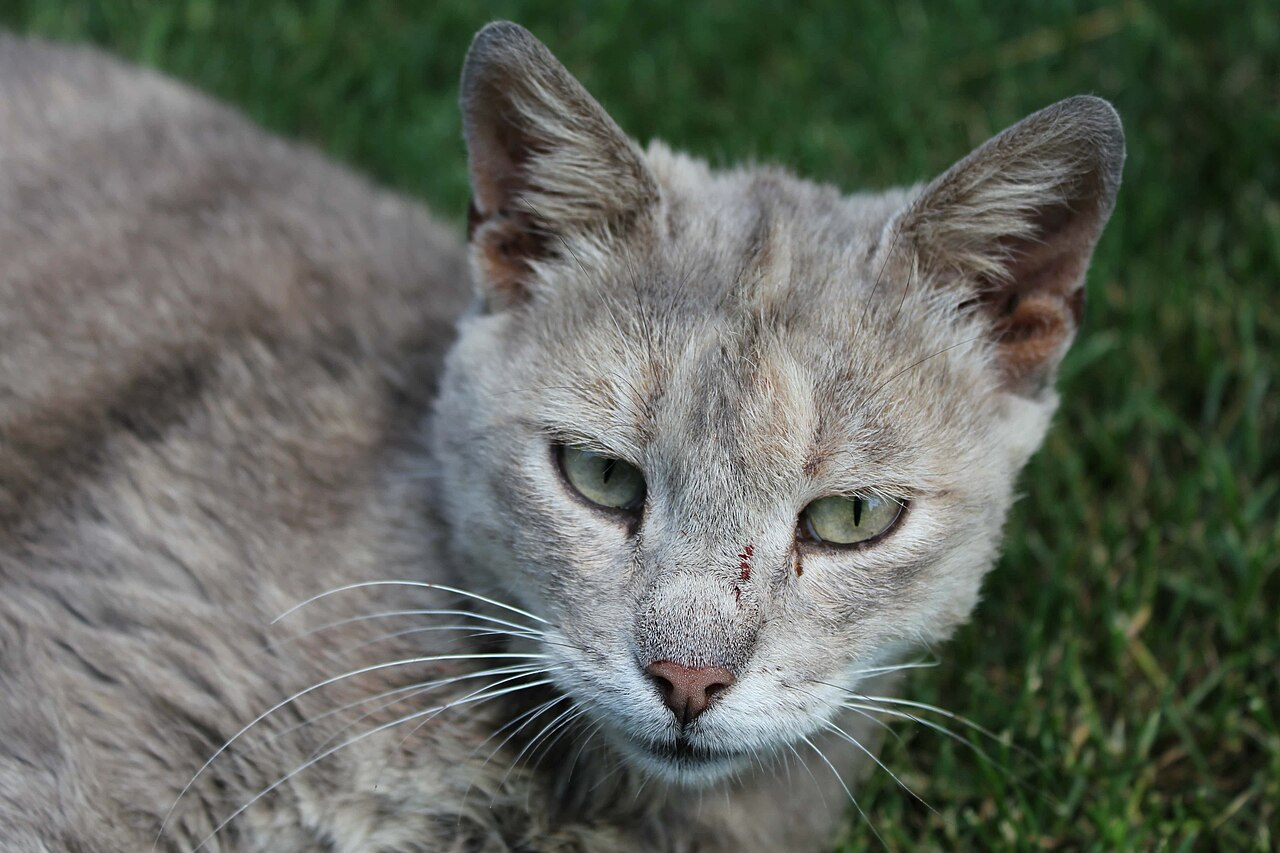
\includegraphics[width=0.7\textwidth]{Diagram/sample-cat.jpg}
    \caption{A single figure. Paths are relative to the graphics root set in \texttt{local\_paths.tex} (default: \texttt{Figures/}).}
    \label{fig:sample-cat}
\end{figure}

\lipsum[7]
